\documentclass{article}

% if you need to pass options to natbib, use, e.g.:
% \PassOptionsToPackage{numbers, compress}{natbib}
% before loading nips_2017
%
% to avoid loading the natbib package, add option nonatbib:
% \usepackage[nonatbib]{nips_2017}


% to compile a camera-ready version, add the [final] option, e.g.:
% \usepackage[final]{nips_2017}

\usepackage[final]{nips_2018}

\usepackage[utf8]{inputenc} % allow utf-8 input
\usepackage[T1]{fontenc}    % use 8-bit T1 fonts
\usepackage{hyperref}       % hyperlinks
\usepackage{url}            % simple URL typesetting
\usepackage{booktabs}       % professional-quality tables
\usepackage{amsfonts}       % blackboard math symbols
\usepackage{nicefrac}       % compact symbols for 1/2, etc.
\usepackage{microtype}      % microtypography
\usepackage{graphicx}

\title{COMP 4211 - Machine Learning Programming Assignment 2 Report}

\author{%
	Cheng Chi Fung \\
	\texttt{cfchengac@connect.ust.hk} \\
}

\begin{document}

\maketitle

\section{CNN Classifier}

\subsection{Screen Shots of the CNN Classifier}
The following are the screen shot of the Predictor Network, CNN Encoder Network and loading the pretrained encoder.

\begin{figure}[h]
  \centering
  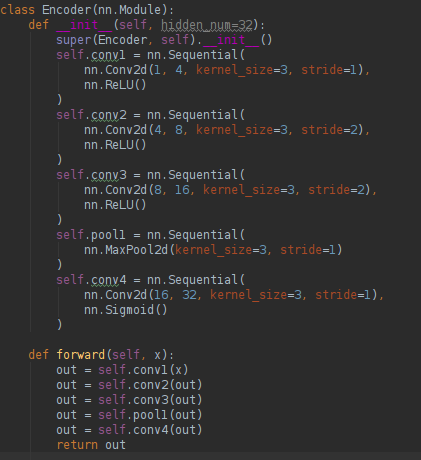
\includegraphics[scale=1]{encoder.png}
  \caption{Screen Shots of Encoder Network}
\end{figure}

\pagebreak

\begin{figure}[h]
  \centering
  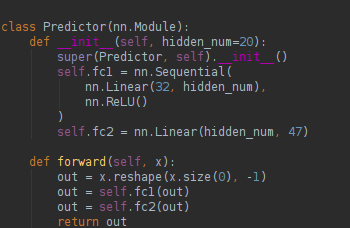
\includegraphics[scale=1]{predictor.png}
  \caption{Screen Shots of Predictor Network}
\end{figure}

\begin{figure}[h]
  \centering
  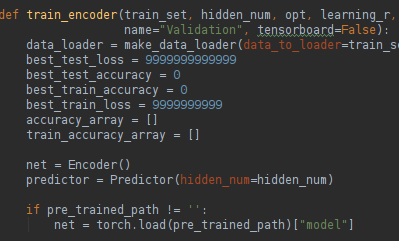
\includegraphics[scale=1]{load_model.png}
  \caption{Screen Shots of Loading Pretrained Encoder Weights}
\end{figure}

\subsection{Hold out validation result of CNN classifier from scratch}

The following are the hold out validation results of CNN classifier from scratch. The network archiecture of using in the hold out validation was the same as the snapshot above. In the validation, we partitioned the training set into the training and validation sets with ratio 4:1. For each candidate set of hyperparameters, we trained the network for $20$ epochs batch size $32$ and validate it against the validation set. The cross entropy loss on validation set shown in the results table was the optimal one .


\begin{table}[htb]
\caption{Hold out Validation Results of scratch CNN classifer}
	\label{sample-table}
	\centering
\begin{tabular}{lllll}
\toprule
		\cmidrule{1-5}
		Parameters set& Optimizer & Learning Rate & Num of Hidden & Cross Entropy Loss 		\\
		\midrule
 			1 & Adam & 0.001 & 32 & 440.98172 \\
 			2 & SGD & 0.1 & 32 &  2533.93441\\
 			3 & SGD & 0.01 & 32 & 2533.97749 \\
 			4 & Adam & 0.001 & 64 & 410.54719 \\
 			5 & SGD & 0.1 & 64 &  2533.96268\\
 			6 & SGD & 0.01 & 64 & 2534.04213 \\
\bottomrule
\end{tabular}
\end{table}

The cross entropy loss of parameters set $4$ had the lowest optimal cross entropy loss $410.54719$ after conducting the hold out validation, so we would choose the parameters set $[Adam, 0.001, 64]$ as the hyperparameters for the training in the testing phase.


\subsection{Hold out validation result of the CNN classifier with Pretrained Encoder Weights}

The following are the hold out validation results of the CNN classifier with pretrained encoder weights. The network archiecture of using in the hold out validation was the same as the snapshot above. In the validation, we partitioned the training set into the training and validation sets with ratio 4:1. For each candidate set of hyperparameters, we trained the network for $20$ epochs batch size $32$ and validate it against the validation set.  The cross entropy loss on validation set shown in the results table was the optimal one .


\begin{table}[htb]
\caption{Hold out Validation Results of CNN classifer with Pretrained Encoder Weights}
	\label{sample-table}
	\centering
\begin{tabular}{lllll}
\toprule
		\cmidrule{1-5}
		Parameters set& Optimizer & Learning Rate & Num of Hidden & Cross Entropy Loss 		\\
		\midrule
 			1 & Adam & 0.001 & 32 & 735.95330 \\
 			2 & SGD & 0.1 & 32 &  668.04426\\
 			3 & SGD & 0.01 & 32 & 964.40623 \\
 			4 & Adam & 0.001 & 64 & 673.44847 \\
 			5 & SGD & 0.1 & 64 &  636.57846\\
 			6 & SGD & 0.01 & 64 & 902.99894 \\
\bottomrule
\end{tabular}
\end{table}

The cross entropy loss of parameters set $5$ had the lowest optimal cross entropy loss $636.57846$ after conducting the hold out validation, so we would choose the parameters set $[SGD, 0.1, 64]$ as the hyperparameters for the training in the testing phase.


\subsection{Testing Results of CNN Classifier}

In the testing phase, for both CNN classifier from scratch and with Pretrained Encoder Weights, we trained using the entire training set with the best set of hyperparameters obtained from the hold out validation and the same network architecture as the hold out validation, and tested with the testing test. We used $32$ as our batch size and trained with $20$ epoch. And we had repeated the same process for $5$ rounds. The below was the results.

\begin{table}[htb]
\caption{Testing Metric of CNN classifier from scratch}
	\label{sample-table}
	\centering
\begin{tabular}{llll}
\toprule
		\cmidrule{1-4}
		& Cross Entropy Loss & Top-1 Accuracy & Top-3 Accuracy 		\\
	\midrule
 	Mean & 515.75526 & 79.27811& 78.79027 \\
 	Std & 12.76076 & 0.34077 & 0.62663\\
\bottomrule
\end{tabular}
\end{table}

\pagebreak

\begin{table}[htb]
\caption{Testing Metric of CNN classifier with Pretrained Encoder Weights }
	\label{sample-table}
	\centering
\begin{tabular}{llll}
\toprule
		\cmidrule{1-4}
		& Cross Entropy Loss & Top-1 Accuracy & Top-3 Accuracy 		\\
	\midrule
 	Mean & 768.54128 & 71.47568 & 70.88601  \\
 	Std & 14.14077 & 0.48995 & 0.37438 \\
\bottomrule
\end{tabular}
\end{table}

The following was the learning curve of the testing metric that we randomly selected only one run out of the total of five runs. The blue color curve was results on testing set and the orange color curve was the results on training set. (The diagram on the left hand side was the results drawn from CNN classifier from scratch and the right hand side was the results drawn from the CNN classifier with Pretrained Encoder Weights )

\begin{figure}[h]
  \centering
  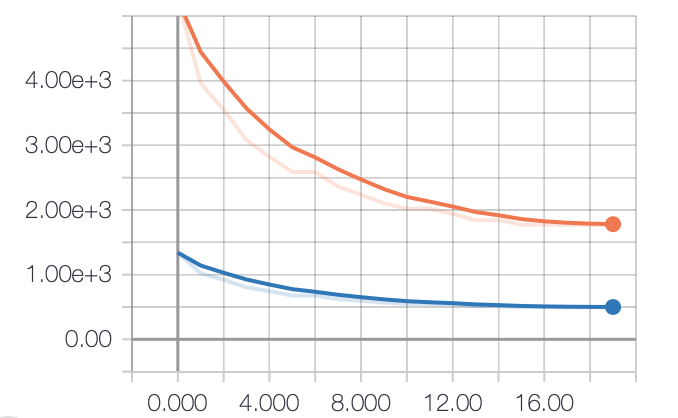
\includegraphics[scale=0.7]{cross_loss_sc.png}
  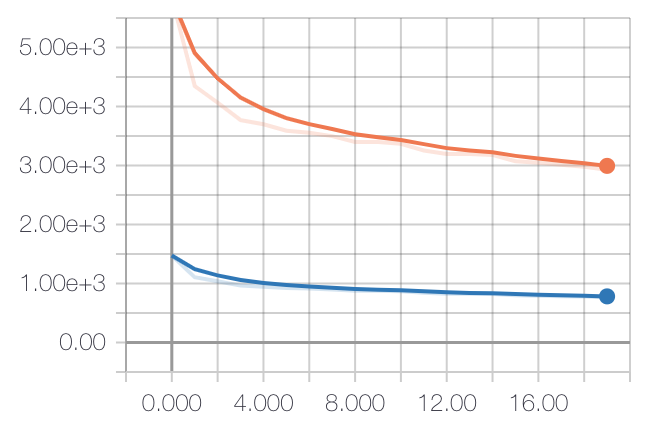
\includegraphics[scale=0.68]{cross_loss_pre.png}
  \caption{Learning Curve of Cross Entropy Loss}
\end{figure}

\pagebreak

\begin{figure}[h]
  \centering
  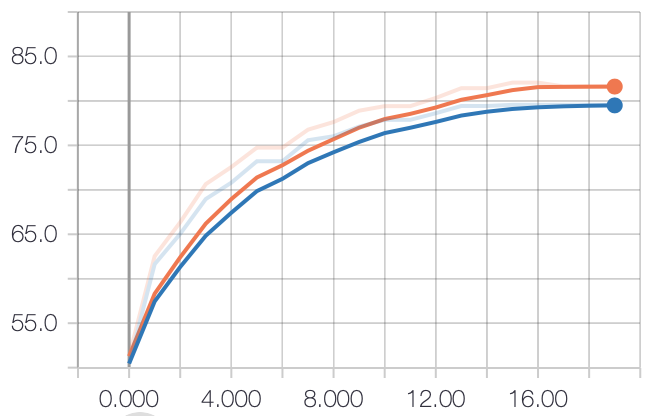
\includegraphics[scale=0.7]{top_1_acc_sc.png}
  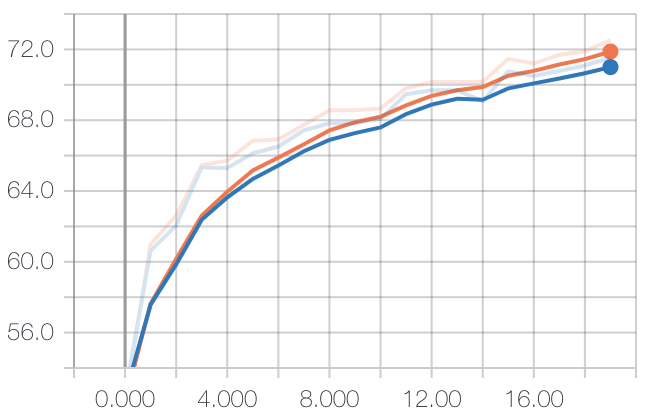
\includegraphics[scale=0.7]{top_1_acc_pre.png}
  \caption{Learning Curve of Top-1 Accuracy}
\end{figure}


\begin{figure}[h]
  \centering
  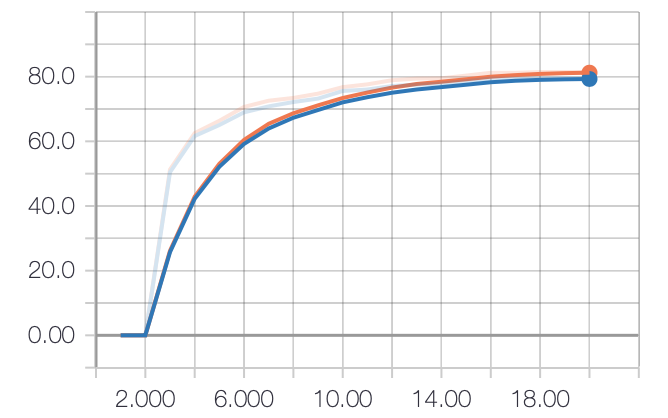
\includegraphics[scale=0.7]{top_3_acc_sc.png}
  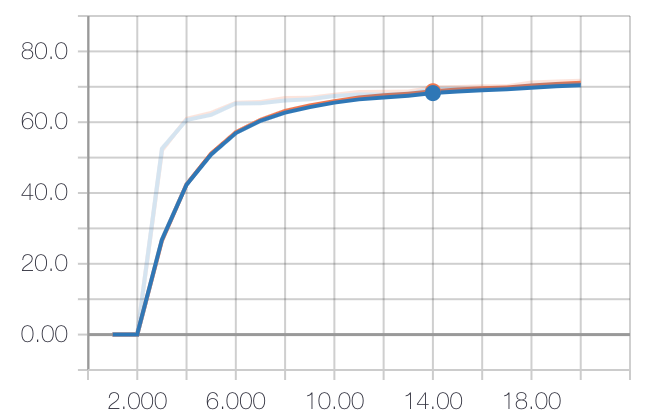
\includegraphics[scale=0.7]{top_3_acc_pre.png}
  \caption{Learning Curve of Top-3 Accuracy}
\end{figure}


\subsection{Analysis on the performance of the CNN classifiers}

Base on the results of the empirical test results, we found out that the pretrained model does help in decreasing \textbf{the training time} and using less epoch. Since, from the results of hold out validation of CNN classifer with Pretrained Weights (Table $2$), we could see the cross entropy loss of validation set that using different set of hyperparameters for training are quite near and low $(902.99-636.57)$. On the other hand, from the results of of hold out validation of CNN classifer without pretrain-ed Weights (Table $1$), we could see the cross entropy loss of using different set of hyper-parameters are quite vary in range $(410.5471-2534.04213)$ and only little of them got low cross entropy loss. Therefore, by using pretrained model, it is far more easier to find good hyper-parameters for final training and hence it reduce for hold out validation and hence helps in decrasing the training time. And this may because the pre-training has already gave the network a head start.

However, the testing results of using the CNN classifier with pretrained weight was not as good as the CNN classifier without pretrained weight. We could see the mean of the \textbf{cross entropy loss, top-1 accuracy and top-3 accuracy} of the CNN without pretrained weight (Table $3$) is better than the CNN with pretrained weight. (Table $4$) with the same number of training epoch. Therefore, once if we could find a good hyparameters for training, the rate of convergence of CNN without pretrained weight is higher than with pretrained weight. This may because the pretraining model making the gradient decent stuck into the local miminma which lower the rate of convergence.



\pagebreak

\section{CAE with Pretrained Encoder}

\subsection{Screen Shots of the CAE with Pretrained Encoder}
The following are the screen shots of the Network of CAE Decoder and loading the pretrained encoder.

\begin{figure}[h]
  \centering
  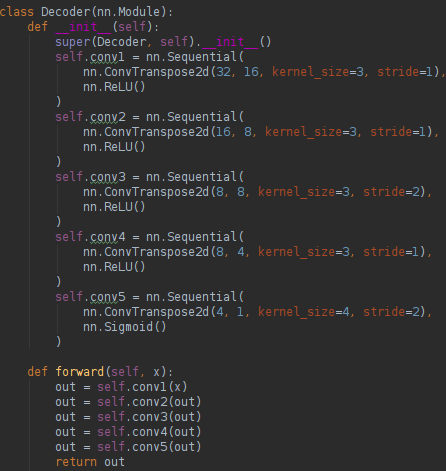
\includegraphics[scale=1]{decoder.png}
  \caption{Screen shot of the Network of CAE Decoder}
\end{figure}

\pagebreak


\begin{figure}[h]
  \centering
  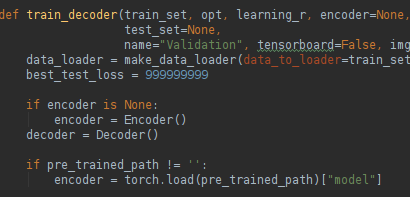
\includegraphics[scale=1]{load_model_de.png}
  \caption{Screen shot of Loading the Pretrained Encoder}
\end{figure}



\subsection{Hold out validation result of CAE with Pretrained Encoder}

The following are the hold out validation results of the CAE with Pretrained Encoder. The network archiecture of using in the hold out validation was the same as the snapshot above. In the validation, we partitioned the training set into the training and validation sets with ratio 4:1. For each candidate set of hyperparameters, we trained the network for $20$ epochs batch size $32$ and validate it against the validation set. The MSE loss of the validation set shown in the results table was the optimal one .


\begin{table}[htb]
\caption{Hold out Validation Results of the CAE with Pretrained Encoder}
	\label{sample-table}
	\centering
\begin{tabular}{llll}
\toprule
		\cmidrule{1-4}
		Parameters set& Optimizer & Learning Rate & MSE Loss\\
		\midrule
 			1 & Adam & 0.01 & 0.02729 \\
 			2 & SGD & 0.1 &  0.03881 \\
 			3 & SGD & 0.01 & 0.11098 \\
\bottomrule
\end{tabular}
\end{table}

Some examples of the image recontructed by the decoder network by using different set of parameters during the hold out validation were shown below.
(The left is the input image and the right is the recontructed image.)

\begin{figure}[h]
  \centering
  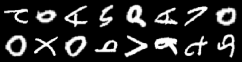
\includegraphics[scale=0.9]{val_raw_round1.png}
  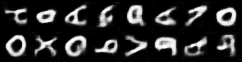
\includegraphics[scale=0.9]{val_recond_round1.png}
  \caption{Parameters set 1}
\end{figure}



\begin{figure}[h]
	\centering
	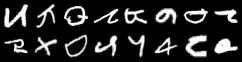
\includegraphics[scale=0.9]{val_raw_round2.png}
	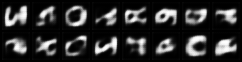
\includegraphics[scale=0.9]{val_recond_round2.png}
	\caption{Parameters set 2}
\end{figure}

\begin{figure}[h]
	\centering
	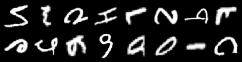
\includegraphics[scale=0.9]{val_raw_round3.png}
	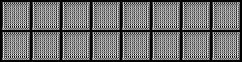
\includegraphics[scale=0.9]{val_recond_round3.png}
	\caption{Parameters set 3}
\end{figure}

\pagebreak

From the results of hold out validation, we could see for parameters set $1$, it had the lowest MSE loss $0.02729$ and the quality of the recontructed image was the best. Therefore, we would choose the parameters set $[Adam, 0.01]$ as the hyperparameters for the training in the testing phase.

\subsection{Testing Results of CAE with Pretrained Encoder}

In the testing phase, we trained using the entire training set with the best set of hyperparameters obtained from the hold out validation and the same network architecture as the hold out validation, and tested with the testing test. We used $32$ as the batch size and trained for $20$ epoch. The following was the results obtained from the testing phase. The MSE Loss shown in the table was the optimal MSE loss.

\begin{table}[htb]
\caption{Testing Result CAE with Pretrained Encoder}
	\label{sample-table}
	\centering
\begin{tabular}{ll}
\toprule
		\cmidrule{1-2}
		& Best MSE Loss	\\
	\midrule
 	& 0.02817 \\
\bottomrule
\end{tabular}
\end{table}


\pagebreak

Some examples of the image recontructed by the decoder network during the test phase were shown below (In the epoch with minimum MSE loss).


\begin{figure}[h]
  \centering
  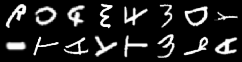
\includegraphics[scale=0.9]{test_raw_image.png}
  \caption{Input Image}
\end{figure}

\begin{figure}[h]
  \centering
  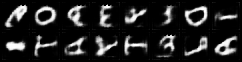
\includegraphics[scale=0.9]{test_recond_image.png}
  \caption{Recontructed Image}
\end{figure}

The following was the learning curve of the MSE loss. The blue color curve was results on testing set and the orange color curve was the results on training set. 

\begin{figure}[h]
  \centering
  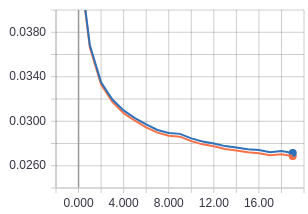
\includegraphics[scale=0.9]{mse_loss_test.png}
  \caption{Recontructed Image}
\end{figure}



\end{document}

